%%%%%%%%%%%%%%%%%%%%%%%%%%%%%%%%%%%%%%%%%%%%%%%%%%%%%%%%%%%%%%%%%%%%%%%%%%%%%%%%
% Medium Length Graduate Curriculum Vitae
% LaTeX Template
% Version 1.2 (3/28/15)
%
% This template has been downloaded from:
% http://www.LaTeXTemplates.com
%
% Original author:
% Rensselaer Polytechnic Institute 
% (http://www.rpi.edu/dept/arc/training/latex/resumes/)
%
% Modified by:
% Daniel L Marks <xleafr@gmail.com> 3/28/2015
%
% Modified by:
% Alberto Botto Poala <alberto.bottopoala@gmail.com> 01/31/2020
%
% Important note:
% This template requires the res.cls file to be in the same directory as the
% .tex file. The res.cls file provides the resume style used for structuring the
% document.
%
%%%%%%%%%%%%%%%%%%%%%%%%%%%%%%%%%%%%%%%%%%%%%%%%%%%%%%%%%%%%%%%%%%%%%%%%%%%%%%%%

%-------------------------------------------------------------------------------
%	PACKAGES AND OTHER DOCUMENT CONFIGURATIONS
%-------------------------------------------------------------------------------

%%%%%%%%%%%%%%%%%%%%%%%%%%%%%%%%%%%%%%%%%%%%%%%%%%%%%%%%%%%%%%%%%%%%%%%%%%%%%%%%
% You can have multiple style options the legal options ones are:
%
%   centered:	the name and address are centered at the top of the page 
%				(default)
%
%   line:		the name is the left with a horizontal line then the address to
%				the right
%
%   overlapped:	the section titles overlap the body text (default)
%
%   margin:		the section titles are to the left of the body text
%		
%   11pt:		use 11 point fonts instead of 10 point fonts
%
%   12pt:		use 12 point fonts instead of 10 point fonts
%
%%%%%%%%%%%%%%%%%%%%%%%%%%%%%%%%%%%%%%%%%%%%%%%%%%%%%%%%%%%%%%%%%%%%%%%%%%%%%%%%

\documentclass[margin]{res}  
% Default font is the helvetica postscript font
\usepackage{helvet}
\usepackage{graphicx}

% Increase text height
\textheight=710pt

%\photo[64pt][0.4pt]{/images/cv.jpeg} 
\begin{document}

%-------------------------------------------------------------------------------
%	NAME AND ADDRESS SECTION
%-------------------------------------------------------------------------------
\name{Alberto Botto Poala}

% Note that addresses can be used for other contact information:
% -phone numbers
% -email addresses
% -linked-in profile

%\address{\\LinkedIn : www.linkedin.com/in/alberto-botto-poala-28291a149
%\\Github : https://www.github.com/Aneesh540\\
%}
\address{}
\address{ \\ \\alberto.bottopoala@gmail.com \\(+49) 176-75328920\\ Via Trento 5, Biella\\ 13900, Italy\\}
%\begin{figure}
%\vspace{+10cm}\hspace{+10cm}
%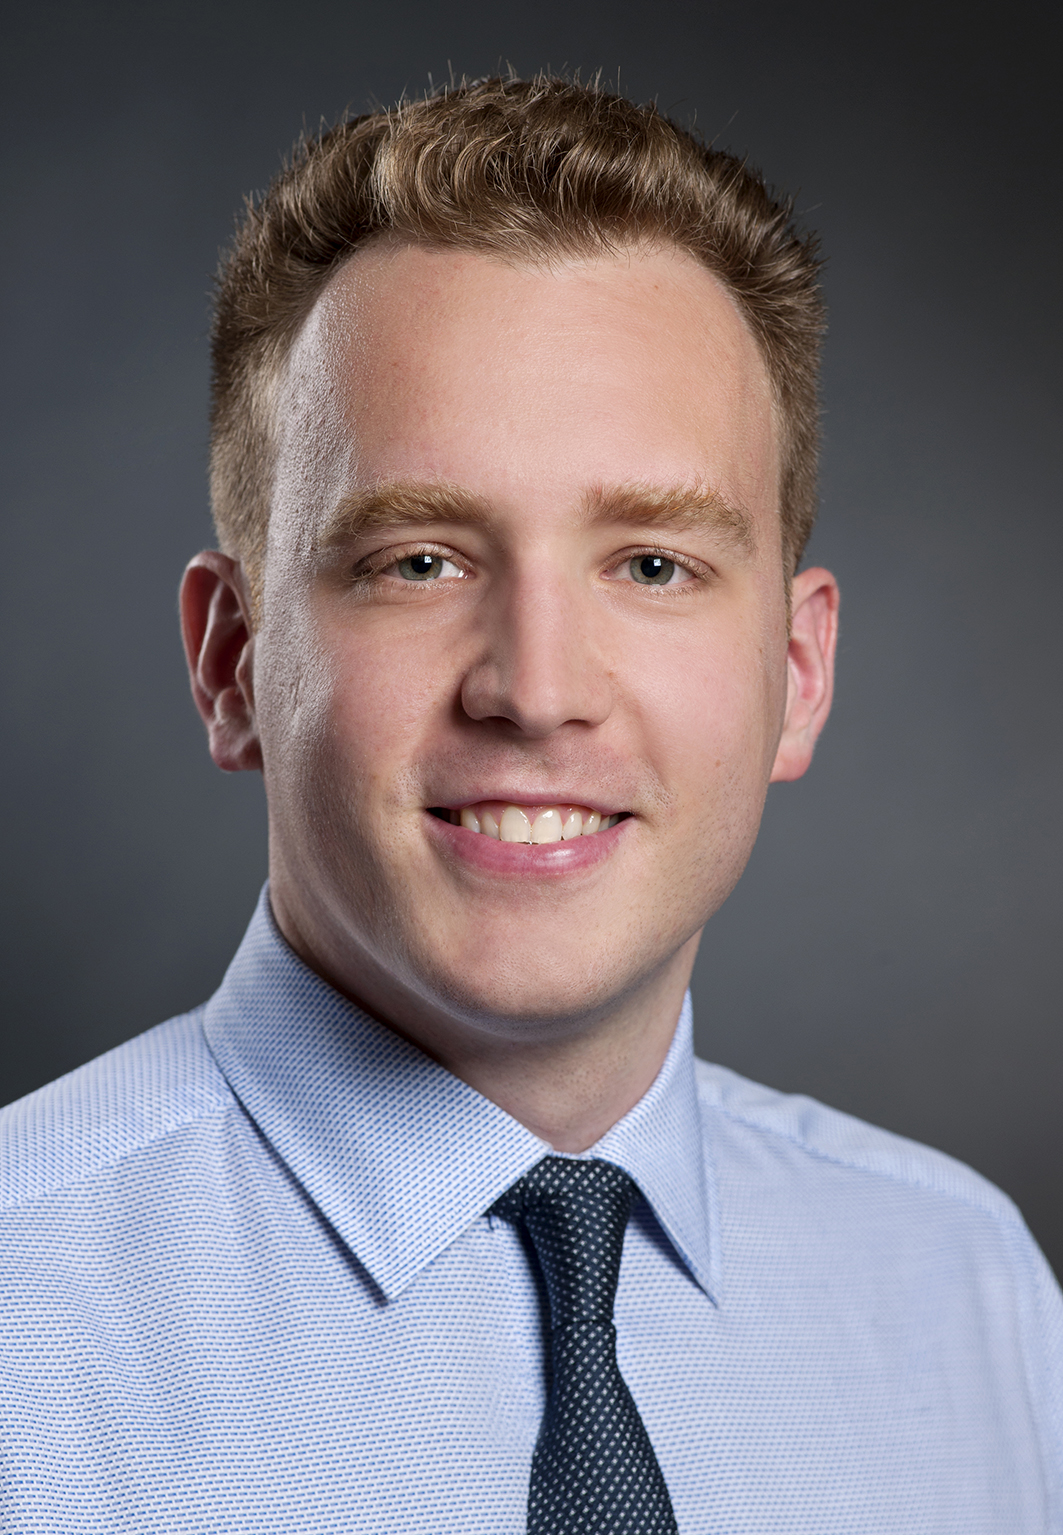
\includegraphics[width=1.15in, height=1.45in]{images/cv.jpeg}
%\end{figure}
% Uncomment to add a third address
%-------------------------------------------------------------------------------

\begin{resume}

%-------------------------------------------------------------------------------
%	EDUCATION SECTION
%-------------------------------------------------------------------------------

\section{PERSONAL DATA}
Born in Biella, Italy\\
DOB 30.12.1990\\
Italian citizenship, unrestricted passport

%-------------------------------------------------------------------------------
%	EDUCATION SECTION
%-------------------------------------------------------------------------------
%\section{OBJECTIVE}
%{\sl Lore Ipsum Pre-Final year B. Tech student at LNMIIT. Inquisitive, hard-working and consistent. Looking for internship opportunities at Microsoft where I can apply my skills and contribute to real-world projects }

\section{EDUCATION}

\textbf{Cadet Pilot Course}\\
{\sl Lufthansa Aviation Training}, May 2018 - May 2020\\
Fully company funded integrated cadet pilot scheme\\
Training locations: BRE, VRB, RLG\\
CPL (LBA)\footnote{CPL, MEP IR and SEP IR will be issued by the German Aviation Authority only after MCC completion (estimate mid-May 2020), now only in possession of PPL (ENAC)}, ATPL theory, MEP IR, SEP IR, PBN credit, RU, VP, MCC\\
300+ hrs total time, 150+ hrs PIC

\textbf{Master of Science, Astrophysics}\\
{\sl Heidelberg Universität}, October 2014 - March 2017\\
Thesis title: \textit{"Hydrodynamic Simulations of Convective Boundary Mixing"}\\
Granted 4 million CPU hours at Jülich Supercomputing Center (JSC)\\
\hfill Final grade: Very Good (1,5)

\textbf{Bachelor of Science, Physics} \\
{\sl Università di Torino}, October 2010 - April 2014\\
Thesis title: \textit{"Combinatory Solutions of 2D Ising Model"}\\
\hfill Final Grade: 108/110

%-------------------------------------------------------------------------------
%	WORKING SECTION
%-------------------------------------------------------------------------------
\section{WORKING EXPERIENCE}

\textbf{Theory Instructor for ATPL(A)}\\
{\sl Aero Club Biella, IT.ATO.0018}, March 2020 - present\\
Ground instructor for POF, RNAV, MAB

\textbf{Visiting Scientist}\\
{\sl Heidelberg Institute for Theoretical Studies}, April 2017 - September 2017\\
Further research on my MS thesis topic with the Physics of Stellar Objects group

\textbf{Parachute Packer}\\
{\sl Dropzone Delta 47}, Summer 2014\\
700+ main canopies packed with no failure

\textbf{Financial Analyst Intern}\\
{\sl Algebrica srl.}, Summer 2013\\
Analysis of arbitrage operations in high frequency trading framework  

%-------------------------------------------------------------------------------
%	PROJECTS SECTION
%-------------------------------------------------------------------------------
\section{SCIENTIFIC CONFERENCES}

\textbf{Compressible Convection Conference 2017}\\
{\sl Université de Lyon}, August 2017\\
Talk title: \textit{"Bulk-Richardson number applications for convective boundary mixing"}  

\bigskip

\pagebreak
\textbf{XIII Würzburg Physics of Stellar Objects Workshop }\\
{\sl Universität Würzburg}, December 2016\\
Talk title: \textit{"Simulating convective boundary layers in astrophysics"}  

\textbf{XII Würzburg Physics of Stellar Objects Workshop}\\
{\sl Universität Würzburg}, July 2016\\
Talk title: \textit{"Simulating convective regimes with SLH"}  
%-------------------------------------------------------------------------------
%	LANGUAGE SKILLS SECTION
%-------------------------------------------------------------------------------

\section{LANGUAGE\\SKILLS}

\textbf{Italian: } mother tongue
\\
\textbf{English: } fluent, ICAO Level 5
\\
\textbf{German: } advanced
\\
\textbf{French: } basic

%-------------------------------------------------------------------------------
%	COMPUTER SKILLS SECTION
%-------------------------------------------------------------------------------
\section{COMPUTER\\SKILLS}

\textbf{General: } Unix, Vim, \LaTeX
\\
\textbf{Languages: } Fortran, Python

%-------------------------------------------------------------------------------
% Modify the format of each position
\begin{format}
\title{l}\\
\dates{l}\location{r}\\
\body\\
\end{format}
%-------------------------------------------------------------------------------

%-------------------------------------------------------------------------------
%	ADDITIONAL ACTIVITIES SECTION
%-------------------------------------------------------------------------------
\section{ADDITIONAL ACTIVITIES}

\normalfont{ \textbf{Skydiving: }USPA B License, 150+ free fall jumps, 5+ hrs tunnel time  \\}
\normalfont{ \textbf{Yoga: }3 years experience \\}

%-------------------------------------------------------------------------------


\end{resume}
\(\)\end{document}
